\chapter{预备知识}

本章节将以规约 \textit{Client\_Server} (图\ref{fig:client_server})为例,
介绍 \TLA 规约的基本结构,以及在寻找归纳不变式过程中的其他预备知识。
\begin{figure}
    \centering
    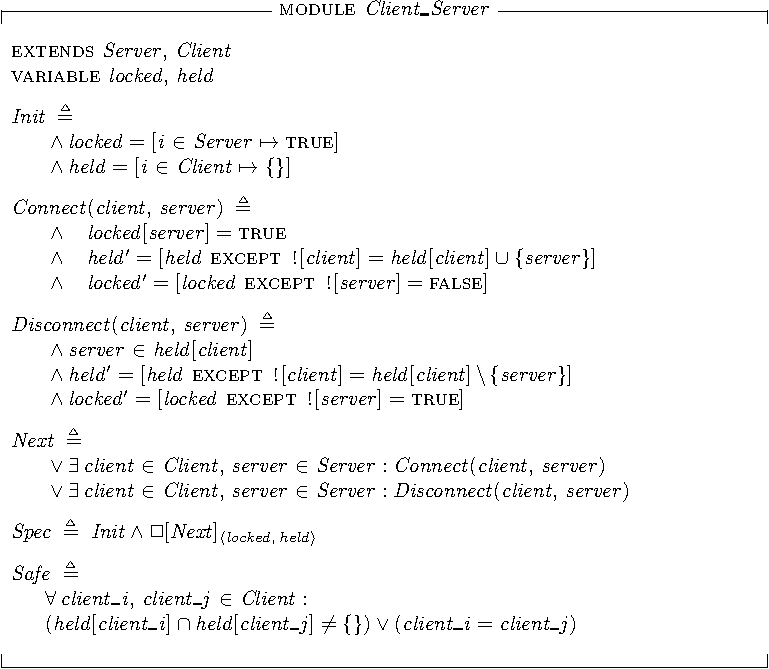
\includegraphics[width=0.8\textwidth]{figures/Client_Server.pdf}
    \caption{Client\_Server 规约}
    \label{fig:client_server}
\end{figure}

\section{\texorpdfstring{TLA\textsuperscript{+}}{TLA+}}
\href{https://lamport.azurewebsites.net/tla/tla.html}{\TLA} \cite{TLA, tla+toolbox}是由计算机科学家 Leslie Lamport 主导开发的,
用于对计算机程序和系统建模,尤其是对并行系统和分布式系统建模的高级语言。
它是基于使用简单的数学语言来精确描述系统行为的理念开发的。
因此,\TLA 的表达方式和一般的编程语言有很大的不同,反而和数学语言更为接近。
\TLA 并不是一种编程语言,而是一种规约语言,它不关注协议或者系统的具体实现,从而能更高层次看到程序整体的设计。
因此,\TLA 及其工具对于消除代码中很难发现和纠错成本高昂的错误非常有用。

需要注意到的是,\TLA 并不是为了寻找归纳不变式而设计的,而是为了对系统进行建模,是为了让规约开发人员能更好地表达一个协议。
它的语法更加丰富,以更加直观的方式表达一个协议。

开发者使用 \TLA 或者其他工具来对分布式协议进行建模的代码,我们将其称之为规约(specification,简称spec)。
图 \ref{fig:client_server} 展示了一个简单的 \TLA 规约,其中包含了一个简单的客户端和服务器的通信协议。
其中两个重要的表达式是 \textit{Init} 和 \textit{Next}。
\textit{Init} 表示系统的初始状态,描述系统最开始时的状态;
而\textit{Next} 则是表示系统的状态是如何转移,也就是系统的状态在每个时间片后会发生怎样的变化。
另一种在自动归纳不变式生成研究中常常使用的工具,IVy,也有相似的语法和结构。
可以看到的是,\TLA 更关注系统的状态和系统状态是发生怎样的转移,对于系统状态转移的具体过程,\TLA 并不关心。
这样的描述方式和状态机非常相似。

\textit{Safety} 是安全属性(safety property),一个正确定义的分布式协议规约,应当在每个可达的状态下都满足安全属性。
这个变量在自动化生成归纳不变式的研究中非常关键。

TLC 是 \TLA 集成的模型检测工具。它的实现方式是通过模拟规约运行的方式,遍历规约中每一个可能的状态和状态转移,
在每个状态下检验安全属性是否成立。
TLC 是一个强大的工具,但是对于复杂的系统,TLC 的运行时间会非常长,这也使得它在证明不变式时,会出现空间爆炸的问题。

除了 TLC 以外,\TLA toolbox\cite{tla+toolbox} 还集成有PlusCal和TLAPS用于命题证明工具,sany用于语法检查工具,
tex 用于将\TLA 美化打印的工具等,这些工具与本文所讨论的问题相关性不高,不展开讨论。

\section{归纳不变式}
验证分布式协议的正确性,就是验证协议定义的安全属性(safety property)是否在每个可达的状态下都成立。
在 \textit{Client\_Server} 规约中,我们可以看到 \textit{Safety} 是一个安全属性,
它表达的是,在任何状态下,如果两个客户端同时连接有同一个服务器,那么这两个客户端是同一个客户端。
换言之,两个不同的客户端不能连接到同一个服务器。

对于简单的系统,即变量和状态不多的系统,我们可以通过遍历每一个可能的状态来验证。
但是对于稍微复杂一些的系统,尤其是越来越多的分布式系统,规模越来越大,状态也越来越复杂。
通过简单的遍历的方式来验证系统的正确性,是不现实的。
寻找一个能够蕴含安全属性的不变式,并且能够在所有可能的状态转移后保持其自身的正确性,这个不变式被称为归纳不变式。
以数学的语言表示为:
\begin{equation}
\begin{aligned}
    &Init \Rightarrow Ind \\
    &Ind \land Next \Rightarrow Ind'\\
    &Ind \Rightarrow Safety
\end{aligned}
\end{equation}
其中$Init$ 是初始状态,$Next$ 是状态转移,$Safety$ 是安全属性,$Ind$ 是归纳不变式,
$Ind'$表达的是这个式子经过状态转移后的状态仍然成立。
也就是说,归纳不变式在规约的初始状态下成立,且从一个状态到另一个状态的转移后,归纳不变式仍然成立。
归纳不变式蕴含安全属性,也就是说,如果归纳不变式成立,那么安全属性也成立。

但是,尤其是对于越复杂的系统而言,寻找归纳不变式并不是一个简单的任务。
实现归纳不变式的自动生成是形式化验证领域一个重要的研究目标。

\section{强化学习}
强化学习(Reinforcement learning, RL)\cite{rl}是机器学习的一个领域,强调如何基于外部环境做出决策,以获得最大化的预期累积奖励。
是区别于监督学习和非监督学习的另外一种基本的机器学习方法。
强化学习的关注点在于寻找对未知领域的探索和对已有知识的利用之间的平衡。
它的目标是通过奖惩来控制智能体完成任务,以获得最大化的预期累积奖励,但程序无需明确告诉智能体如何完成任务。

在机器学习问题中,环境通常被抽象为马尔可夫决策过程(Markov decision processes,MDP)\cite{markov},
因为很多强化学习算法在这种假设下才能使用动态规划的方法。
传统的动态规划方法和强化学习算法的主要区别是,后者不需要关于MDP的知识,而且针对无法找到确切方法的大规模MDP。

\begin{figure}
    \centering
    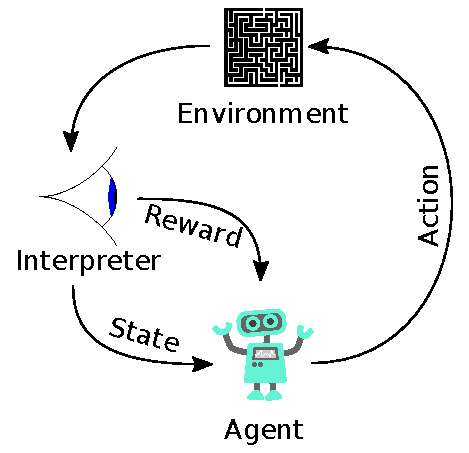
\includegraphics[width=0.6\textwidth]{figures/Reinforcement_learning_diagram.pdf}
    \caption{强化学习框架}
    \label{fig:rl}
\end{figure}
图 \ref{fig:rl} 展示了强化学习的框架。
强化学习中,主要是智能体(agent)和环境(environment)之间的交互。
智能体,可以感知环境的状态(State),并根据反馈的奖励(Reward)学习选择一个合适的动作(Action),来最大化长期总收益。
环境是智能体所处的环境,它会根据智能体的动作,给予智能体奖励,并作出状态转移,智能体根据奖励和环境状态的变化来调整自己的策略。
实现强化学习的策略算法有很多,其中最著名的有 Deep Q Network(DQN)\cite{dqn},Q-learning\cite{q-learning}等。

在本文的项目中,我们使用强化学习的方法来加速归纳不变式的生成。
我们使智能体理解\TLA 原文件的内容,让智能体合理选择生成归纳不变式的种子(seed),
并将每一次智能体选择的种子所生成的不变式的检验结果反馈给智能体,包括反例的数量,内容和生成时间等。
智能体根据这些反馈信息,调整自己的策略,以便更快地找到一个满足安全属性的归纳不变式。

\section{Apalache}
Apalache\cite{apalache1, apalache2} 是一个面向\TLA 规约的模型检查器(model checker)。
与 TLC 不同的是,Apalache 并不是通过遍历所有可能的状态来检验安全属性是否成立,而是通过 SMT solver 来检验,
而是将\TLA 规约转换为 SMT 问题,然后使用 SMT solver (如Z3\cite{z3})求解来检验安全属性是否成立。
Apalaches 是一种符号检查器,它和 SMT solver 一样基于逻辑推理和公式求解实现的。
故而,Apalache相较于TLC,更适合用于归纳不变式的搜索和验证工作。
Apalache 对\TLA 源文件的语法中引入了一些限制,
尽管没有完全支持\TLA 的所有语法,但是这方便了 SMT 求解器进行求解。

\TLA 是一个“弱类型”的编程语言,它对变量没有严格的类型著名。
但是,Apalache 需要了解\TLA 规约中变量的类型才能工作。
尽管 Apalache 有一套自己的类型推断系统,但是,它并不能完全解决所有的类型推断问题。
这使得用户,对于某些协议,需要以注释的形式来提供变量的类型。

